%
% fourierkoef.tex -- Bestimmung der Fourier-Koeffizienten
%
% (c) 2018 Prof Dr Andreas Müller, Hochschule Rapperswil
%
\section{Fourier-Koeffizienten}
\rhead{Fourier-Koeffizienten}
In diesem Abschnitt bestimmen wir die Fourierkoeffizienten für ein
trigonometrisches Polynom der Form
\begin{equation}
p_n(t)
=
a_0 + \sum_{k=1}^{n-1} a_k\cos kt + \sum_{k=1}^{n-1} b_k\sin kt + a_n\cos nt,
\label{skript:fourier:ansatz}
\end{equation}
derart, dass die Werte
\begin{equation}
y_j \quad\text{zu den Zeitpunkten}\quad t_j=2\pi\frac{j}{N},\qquad 1\le j< N
\label{skript:fourier:gleichungen}
\end{equation}
möglichst genau die Funktionswerte $p_n(t_j)$ reproduzieren.

Im Ansatz~\eqref{skript:fourier:ansatz} für $p_n(t)$ finden wir
genau $2n$ zu bestimmende Koeffizienten, nämlich $a_0$,
$n$ Koeffizienten $a_k$ mit $k=1,\dots,n$
und $n-1$ Koeffizienten $b_k$ mit $k=1,\dots,n-1$.
Mit $N$ Datenpunkten $y_j$ haben wir genau die $N$ Bedingungen
$p_n(t_j)=y_j$, um diese Koeffizienten zu bestimmen.
Die Bedingungen $p_n(t_j)=y_j$ sind $N$ lineare Gleichungen für die
$2n$ Koeffizienten, sie dürften sich also genau dann exakt lösen
lassen, wenn $N=2n$, wenn also die Zahl der Datenpunkte gerade ist.

Für $N<2n$ haben wir weniger Gleichungen als Koeffizienten, es ist
also unmöglich, die Koeffizienten ohne zusätzliche Annahmen zu bestimmen.
Das Problem ist also nur dann überhaupt lösbar, wenn $N\ge 2n$ ist.
Für $N>2n$ haben wir zu viele Daten, wir können nicht erwarten, dass
das Gleichungssystem $p_n(t_j)=y_j$ überhaupt eine Lösung hat.
Im optimalen Fall, für $N=2n$ sollte es möglich sein, die Koeffizienten so
zu bestimmen, dass die Funktionswerte $y_j$ exakt reproduziert werden.

\subsection{Least Squares}
Für $N>2n$ können wir nicht erwarten, dass der Ansatz
\eqref{skript:fourier:ansatz} die Daten exakt reproduzieren kann,
wir müssen uns also mit einer Näherungslösung begnügen.
Wir verlangen stattdessen, dass der Fehler der Lösung möglichst gering
wird, dass also
\[
L=L(a_0,a_1,\dots,a_n,b_1,\dots,b_{n-1})= \sum_{j=1}^N (y_j - p_n(t_j))^2
\]
möglichst klein wird.

Die Grösse $L$ wird minimal, wenn alle Ableitungen nach den Koeffizienten
verschwinden:
\begin{equation}
\frac{\partial L}{\partial a_0}=0,
\qquad
\frac{\partial L}{\partial a_l}=0, \;{1\le l\le n}
\qquad
\frac{\partial L}{\partial b_l}=0, \;{1\le l\le n-1}
\label{skript:fourier:leastsquaresableitungen}
\end{equation}
Um die Koeffizienten zu bestimmen, müssen wir die Ableitungen in
\eqref{skript:fourier:leastsquaresableitungen}
berechnen und erhalten die Gleichungen
\begin{align}
\frac{\partial L}{\partial a_0}
&=
-2 \sum_{j=1}^N (y_j-p_n(t_j))\cdot \frac{\partial p_n}{\partial a_0}(t_j)=0,
&&
\label{skript:fourier:a0ableitung}
\\
\frac{\partial L}{\partial a_l}
&=
-2 \sum_{j=1}^N (y_j-p_n(t_j))\cdot \frac{\partial p_n}{\partial a_l}(t_j)=0
&k&=1,\dots,n,
\label{skript:fourier:akableitung}
\\
\frac{\partial L}{\partial b_l}
&=
-2 \sum_{j=1}^N (y_j-p_n(t_j))\cdot \frac{\partial p_n}{\partial b_l}(t_j)=0
&k&=1,\dots,n-1.
\label{skript:fourier:bkableitung}
\end{align}
Man beachte, dass $p_n(t_j)$ die Koeffizienten $a_0$, $a_k$ und $b_k$
linear enthält.
Der erste Klammerausdruck $y_j-p_n(t_j)$ in der Summe enthält daher die
Koeffizienten ebenfalls nur linear, die Ableitungen nach den Koeffizienten
enhalten daher die Koeffizienten überhaupt nicht mehr.
Tatsächlich ergibt die Berechnung der Ableitungen
\begin{align}
\frac{\partial p_n}{\partial a_0}(t_j)
&=
1
&&
\label{skript:fourier:a0abl}
\\
\frac{\partial p_n}{\partial a_l}(t_j)
&=
\cos lt_j
&l&=1,\dots,n
\label{skript:fourier:akabl}
\\
\frac{\partial p_n}{\partial b_l}(t_j)
&=
\sin lt_j
&l&=1,\dots,n-1.
\label{skript:fourier:bkabl}
\end{align}
\definecolor{darkblue}{rgb}{0,0,0.6}%
Setzen wir diese Ableitungen als {\color{darkblue}dunkelblaue} Terme in
\eqref{skript:fourier:a0ableitung}--\eqref{skript:fourier:bkableitung} ein
und vertauschen die Reihenfolge der Summationen über $k$ und $j$,
erhalten wir die Gleichungen
\definecolor{darkred}{rgb}{0.6,0,0}%
\begin{equation}
\left.
\begin{aligned}
0&=
\sum_{j=1}^N
\biggl(
y_j - a_0 - \sum_{k=1}^n a_k\cos kt_j - \sum_{k=1}^{n-1} b_k\sin kt_j
\biggr)\cdot\mathstrut{\color{darkblue}1}
\\
&=
\sum_{j=1}^N y_j
-Na_0
-\sum_{k=1}^n a_k {\color{darkred}\sum_{j=1}^N\cos kt_j}
-\sum_{k=1}^{n-1} b_k {\color{darkred}\sum_{j=1}^N\sin kt_j},
\\
0&=
\sum_{j=1}^N
\biggl(
y_j - a_0 - \sum_{k=1}^n a_k\cos kt_j - \sum_{k=1}^{n-1} b_k\sin kt_j
\biggr)\cdot\mathstrut {\color{darkblue}\cos lt_j}
\\
&=
\sum_{j=1}^N y_j \cos lt_j
-a_0\sum_{j=1}^N \cos lt_j
-\sum_{k=1}^n a_k {\color{darkred}\sum_{j=1}^N\cos kt_j\cos lt_j}
-\sum_{k=1}^{n-1} b_k {\color{darkred}\sum_{j=1}^N\sin kt_j\cos lt_j},
%&l&=1,\dots,n-1
\\
0
&=
\sum_{j=1}^N
\biggl(
y_j - a_0 - \sum_{k=1}^n a_k\cos kt_j \sum_{k=1}^{n-1} b_k\sin kt_j
\biggr)\cdot\mathstrut {\color{darkblue}\sin lt_j}
\\
&=
\sum_{j=1}^N y_j \sin lt_j
-a_0\sum_{j=1}^N \sin lt_j
-\sum_{k=1}^n a_k {\color{darkred}\sum_{j=1}^N\cos kt_j\sin lt_j}
-\sum_{k=1}^{n-1} b_k {\color{darkred}\sum_{j=1}^N\sin kt_j\sin lt_j}.
%&l&=1,\dots,n
\end{aligned}
\right\}
\label{skript:fourier:gl2}
\end{equation}
Hier haben wir die Faktoren $-2$ ebenfalls weggelassen.
Auf den ersten Blick scheinen diese Gleichungen nicht einfach lösbar zu
sein, die {\color{darkred}dunkelrot} hervorgehobenen Koeffizienten der
Unbekannten $a_0$, $a_k$ und $b_k$ scheinen ziemlich kompliziert zu sein.
Es stellt sich aber heraus, dass diese direkt ausgewertet werden können,
was im nächsten Abschnitt geschehen soll.

\subsection{Trigonometrische Summen}
In den Gleichungen~\eqref{skript:fourier:gl2} treten als Koeffizienten
für die Unbekannteno $a_0$, $a_k$ und $b_k$ trigonometrische Summen
der Form
\begin{equation}
\sum_{j=1}^N \cos kt_j
\qquad
\text{oder}
\qquad
\sum_{j=1}^N \sin kt_j,
\label{skript:fourier:trigosum}
\end{equation}
sowie Summen von Produkten trigonmetrischer Funktionen wie
\begin{equation}
\sum_{j=1}^N \cos kt_j\cos lt_j,\quad
\sum_{j=1}^N \cos kt_j\sin lt_j
\quad
\text{oder}
\quad
\sum_{j=1}^N \sin kt_j\sin lt_j
\label{fourier:produkte}
\end{equation}
auf.
In diesem Abschnitt sollen diese Summen mit Hilfe einer geometrischen
Überlegung berechnet werden.

Wir befassen uns zunächst mit Summen der Form
\eqref{skript:fourier:trigosum} und beweisen den folgenden Satz.

\begin{figure}
\centering
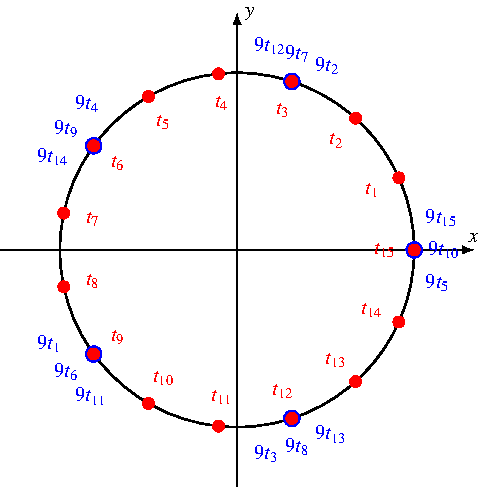
\includegraphics{chapters/6/trigosum.pdf}
\caption{Verteilung der Punkte $(\cos t_j, \sin t_j)$  auf dem Einheitskreis 
in rot.
Die Punkte $(\cos kt_j,\sin kt_j)$ für $k=9$ bilden eine Teilmenge, die
blau dargestellt ist.
Jeder blaue Punkt wird genau dreimal besucht, sie bilden ein gleichseitiges
Fünfeck mit den Punkten $(\cos 3t_j,\sin 3t_j)$ als Ecken.
Deren Schwerpunkt ist wieder der Nullpunkt.
\label{fourier:einheitskreis}
}
\end{figure}

\begin{satz}
\label{skript:fourier:orthogonalitaet1}
Ist $t_j=2\pi j/N$, dann gelten für beliebige ganze Zahlen $l$,
mit $0\le l\le n$, die Identitäten
\begin{equation*}
\begin{aligned}
\sum_{j=1}^N \cos lt_j
&=
\begin{cases}
N&\qquad l=0\\
0&\qquad\text{sonst}
\end{cases}
\\
\sum_{j=1}^N \sin lt_j
&=0.
\end{aligned}
\end{equation*}
\end{satz}

\begin{proof}[Beweis]
Wir betrachten zunächst den Fall $l=0$.
In diesem Fall ist $\cos lt_j=1$ und $\sin lt_j=0$ und damit
\[
\sum_{j=1}^N \cos lt_j = N
\qquad\text{und}\qquad
\sum_{j=1}^N \sin lt_j = 0.
\]
Im Folgenden können wir daher annehmen, dass $l\ne 0$.

In Abbildung~\eqref{fourier:einheitskreis} kann man sehen, dass die Punkte
$(\cos t_j,\sin t_j)$ auf dem Einheitskreis ein regelmässiges Polygon
mit $N$ Ecken bilden.
Der Schwerpunkt des Polygons ist ganz offensichtlich der Mittelpunkt.
Daraus folgt
\[
\sum_{j=1}^N \cos t_j = 0
\qquad\text{und}\qquad
\sum_{j=1}^N \sin t_j = 0.
\]
Damit ist der Satz für den Fall $l=1$ bewiesen.

Für beliebiges $l\ne 0$ beobachten wir, dass die Punkte 
$(\cos lt_j,\sin lt_j)$ eine Teilmenge der Punkte $(\cos t_j, \sin t_j)$
sind.
Wenn $l$ und $N$ teilerfremd sind, sind die Mengen gleich.
Wenn $l$ und $N$ dagegen den grössten gemeinsamen Teiler
$r=\operatorname{ggT}(l,N)$ haben, dann
ist die Menge 
\[
\{ 
(\cos lt_j,\sin lt_j)\,|\,j=1,\dots,N
\}
=
\{
(\cos rt_j,\sin rt_j)\,|\,j=1,\dots,N/r
\}
\]
ein regelmässiges Polygon mit $N/r$ Ecken.
Diese Situation ist in Abbildung~\ref{fourier:einheitskreis} mit den
blauen Punkten für den Fall $r=3=\operatorname{ggT}(9,15)$
illustriert.
Wie im Falle von $l=1$ folgt\footnote{Etwas formeller könnten wir sagen,
dass wir hier vollständige Induktion nach $N$ machen.
Was wir im letzten Schritt nämlich brauchen ist der Wert einer
trigonometrischen Summe mit $N/r<N$ Summanden, deren Werte wir gemäss
der naheligenden Induktionsannahme bereits kennen.},
dass der Schwerpunkt des Polygons der
Nullpunkt ist, und damit, dass
\begin{align*}
\sum_{j=1}^N \cos lt_j 
=
\sum_{j=1}^N \cos rt_j 
=
0,
\\
\sum_{j=1}^N \sin lt_j 
=
\sum_{j=1}^N \sin rt_j 
=
0.
\end{align*}
Damit ist alles gezeigt.
\end{proof}

In \eqref{fourier:produkte} werden die Summen von Produkten benötigt.
Mit üblichen trigonometrischen Umformungen kann man diese in Summen
von einfachen trigonometrischen Funktionen umwandeln.
Wir verwenden dazu die Formeln
\begin{align}
\cos\alpha\cos\beta
&=
\frac12\bigl(\cos(\alpha-\beta)+\cos(\alpha+\beta)\bigr),
\label{fourier:coscos}
\\
\sin\alpha\sin\beta
&=
\frac12\bigl(\cos(\alpha-\beta) + \cos(\alpha+\beta)\bigr).
\label{fourier:sinsin}
\\
\sin\alpha\cos\beta
&=
\frac12\bigl(\sin(\alpha-\beta) + \sin(\alpha+\beta)\bigr),
\label{fourier:sincos}
\end{align}
Damit können wir die Summen in \eqref{fourier:produkte} umwandeln:
\begin{align*}
\sum_{j=1}^N \cos kt_j\cos lt_j
&=
\sum_{j=1}^N \frac12\bigl(\cos (k-l)t_j +\cos(k+l)t_j\bigr)
\\
&=
\frac12\sum_{j=1}^N \cos (k-l)t_j
+ \frac12\underbrace{\sum_{j=1}^N\cos(k+l)t_j}_{\displaystyle=0}
\\
&=
\begin{cases}
\displaystyle\frac{N}2&\qquad k=l\\
0&\qquad\text{sonst}
\end{cases}
\\
\sum_{j=1}^N \sin kt_j \sin lt_j
&=
\sum_{j=1}^N \frac12\bigl(\cos(k-l)t_j +\cos(k+l)t_j\bigr)
\\
&=\frac12\sum_{j=1}^N \cos(k-l)t_j
+\frac12\underbrace{\sum_{j=1}^N \cos(k+l)t_j}_{\displaystyle=0}
\\
&=
\begin{cases}
\displaystyle\frac{N}2&\qquad k=l\\
0&\qquad\text{sonst}
\end{cases}
\\
\sum_{j=1}^N \sin kt_j \cos lt_j
&=
\sum_{j=1}^N \frac12\bigl(\sin(k-l)t_j +\sin(k+l)t_j\bigr)
\\
&=
\frac12\underbrace{\sum_{j=1}^N \sin(k-l)t_j}_{\displaystyle=0}
+
\frac12\underbrace{\sum_{j=1}^N \sin(k+l)t_j}_{\displaystyle=0}
=0.
\end{align*}
Damit haben wir den folgenden Satz bewiesen:

\begin{satz}
\label{skript:fourier:satzprodukte}
Für beliebige $k,l\in \mathbb N$ gilt
\begin{align*}
\sum_{j=1}^N
\cos kt_j \cos lt_j
&=
\begin{cases}
N                     &\qquad k=l=0\\
\displaystyle\frac{N}2&\qquad k=l > 0\\
0                     &\qquad\text{sonst}
\end{cases}
\\
\sum_{j=1}^N
\sin kt_j \sin l_j
&=
\begin{cases}
\displaystyle \frac{N}2&\qquad k=l\\
0                      &\qquad\text{sonst}
\end{cases}
\\
\sum_{j=1}^N
\sin kt_j \cos lt_j
&=
0
\end{align*}
\end{satz}
Mit dem Kronecker-$\delta$ 
\index{Kronecker-$\delta$}%
\[
\delta_{kl}
=
\begin{cases}
1&\qquad k=l\\
0&\qquad\text{sonst}
\end{cases}
\]
können wir die ersten zwei Formeln für $k,l>0$ noch etwas kompakter 
als
\begin{equation}
\sum_{j=1}^N
\cos kt_j \cos lt_j
=
\sum_{j=1}^N
\sin kt_j \sin l_j
=
\delta_{kl}\frac{N}2
\label{skript:fourier:trigsumsummary}
\end{equation}
schreiben.

In den folgenden Abschnitten verwenden wir diese Formeln, um die
Koeffizienten $a_k$ und $b_k$ zu bestimmen.
Der Koeffizient $a_0$ muss gesondert behandelt werden.

\subsection{Bestimmung von $a_0$}
In der Gleichung
\[
0
=
\sum_{j=1}^Ny_j
-Na_0
-\sum_{k=1}^na_k\underbrace{\sum_{j=1}^N\cos kt_j}_{\displaystyle=0}
-\sum_{k=1}^nb_k\underbrace{\sum_{j=1}^N\sin kt_j}_{\displaystyle=0}
\]
verschwinden die trigonometrischen Summen über $j$ nach
Satz~\ref{skript:fourier:orthogonalitaet1} und es bleibt die Gleichung
\begin{align*}
0
&=
\sum_{j=1}^Ny_j
-Na_0
\\
\Rightarrow\qquad
a_0&=\frac1{N}\sum_{j=1}^N y_j.
\end{align*}
Der Koeffizient $a_0$ ist der Mittelwert der Werte $y_j$.

\subsection{Bestimmung von $a_k, k>0$}
Zur Bestimmung von $a_k$ mit $k>0$ müssen wir die Gleichung
\[
0
=
\sum_{j=1}^N y_j\cos lt_j
-
a_0\underbrace{\sum_{j=1}^N\cos lt_j}_{\displaystyle=0}
-\sum_{k=1}^na_k\sum_{j=1}^N\cos kt_j\cos lt_j
-\underbrace{\sum_{k=1}^nb_k\sum_{j=1}^N\sin kt_j\cos lt_j}_{\displaystyle=0}
\]
heranziehen.
Die zweite und vierte Summe verschwindet wegen
Satz~\ref{skript:fourier:satzprodukte}, so dass wir die die Gleichung
\begin{align*}
0&=
\sum_{j=1}^N y_j\cos lt_j
-\sum_{k=1}^na_k\sum_{j=1}^N\cos kt_j\cos lt_j
\end{align*}
erhalten.
Die innere Summe über $j$ im zweiten Term verschwindet, wieder gemäss 
Satz~\ref{skript:fourier:satzprodukte}, für alle Werte
von $k$ ausser für $k=l$, in diesem Fall ist sie $N/2$. 
Damit können wir nach $a_k$ auflösen:
\begin{align*}
0&
=
\sum_{j=1}^N y_j\cos lt_j
-\sum_{k=1}^na_k\delta_{kl}\frac{N}2
=
\sum_{j=1}^N y_j\cos lt_j
-a_l\frac{N}2
\\
\Rightarrow\qquad 
a_l &= \frac{2}{N}\sum_{j=1}^Ny_j\cos lt_j.
\end{align*}

\subsection{Bestimmung von $b_k$}
Zur Bestimmung von $b_k$ müssen wir die Gleichung
\[
0=\sum_{j=1}^N y_j\sin lt_j 
-a_0\sum_{j=1}^N \sin lt_j
-\sum_{k=1}^na_k\sum_{j=1}^N\cos kt_j\sin lt_j
-\sum_{k=1}^nb_k\sum_{j=1}^N\sin kt_j\sin lt_j
\]
heranziehen.
Nach Satz~\ref{skript:fourier:satzprodukte}
verschwindet die zweite und die dritte Summe 
und in der letzten Summe
verschwinden alle Terme ausser der Term mit $k=l$, für den die
innere Summe über $j$ den Wert $N/2$ hat.
Damit wird die Gleichung vereinfacht zu
\begin{align*}
0
&=
\sum_{j=1}^Ny_j\sin lt_j - \sum_{k=1}^{n-1}b_l\delta_{kl}\frac{N}2
=
\sum_{j=1}^Ny_j\sin lt_j - b_l\frac{N}2
\\
\Rightarrow\qquad
b_l
&=
\frac{2}{N}\sum_{j=1}^Ny_j\sin lt_j.
\end{align*}

\subsection{Zusammenstellung der Resultate}
Sei $N=2n$ eine gerade natürliche Zahl.
Eine $2\pi$-periodische Funktion $f(t)$ kann als trigonometrisches Polynom
der Form
\[
p_n(t)
=
a_0 + \sum_{k=1}^{n-1} (a_k\cos kt + b_k\sin kt) + a_n\cos nt
\]
derart approximiert werden, dass zu den Zeiten $t_j=2\pi j/N, j=1,\dots,N$ 
die Funktion und das trigonometrische Polynom übereinstimmen:
\[
f(t_j) = y_j = p_n(t_j).
\]
Dazu müssen die Koefizienten
\begin{align*}
a_0
&=
\frac{1}N
\sum_{j=1}^N y_j,
\\
a_k
&=
\frac{2}N
\sum_{j=1}^N y_j\cos t_j
=
\frac{2}N
\sum_{j=1}^N y_j\cos \frac{2\pi j}{N}&\text{für }k&=1,\dots,n
\\
\text{und}\qquad
b_k
&=
\frac{2}N
\sum_{j=1}^N y_j\sin t_j
=
\frac{2}N
\sum_{j=1}^N y_j\sin \frac{2\pi j}{N}&\text{für }k&=1,\dots,n-1,
\end{align*}
verwendet werden.

\subsection{Beispiel: Dreiecksfunktion\label{subsection:fourier:dreiecksfunktion}}
\begin{figure}
\centering
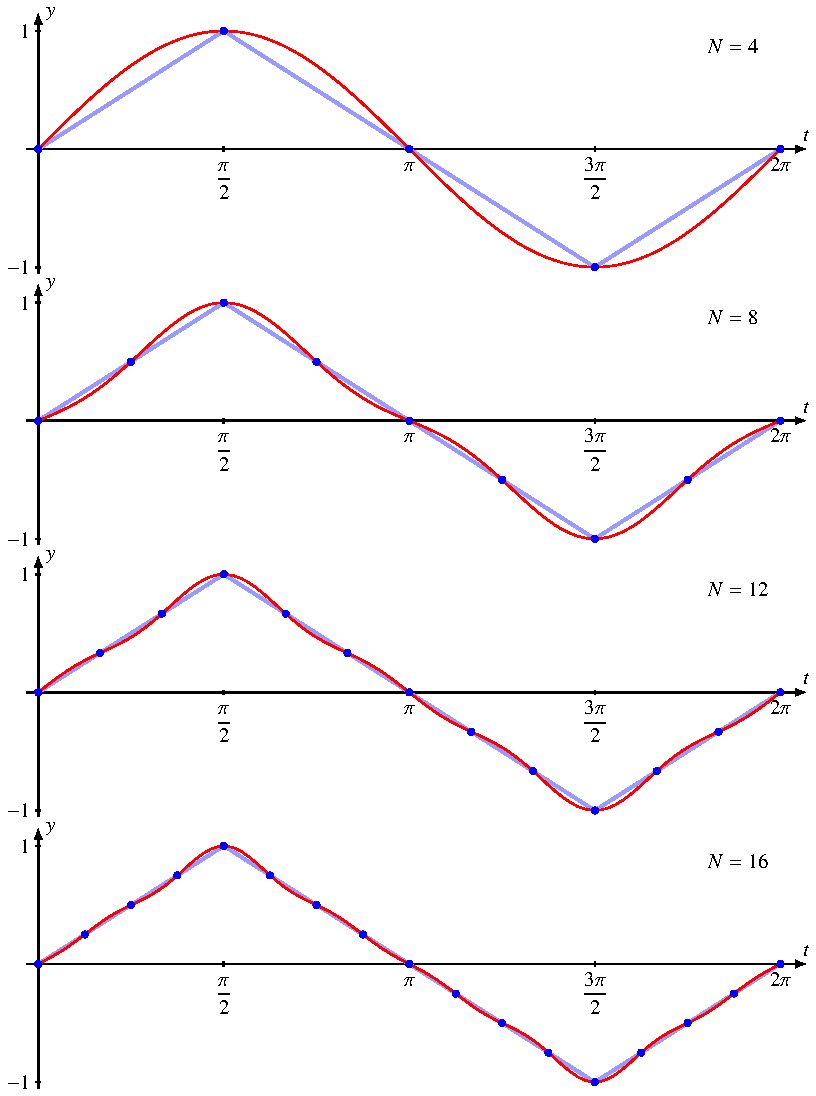
\includegraphics{chapters/6/dreieck.pdf}
\caption{Dreiecksfunktion ({\color{blue}blau}) approximiert mit
trigonometrischen Polynomen  $p_n(t)$ ({\color{red}rot})
mit verschiedenen Werten von $N=2n$.
\label{skript:fourier:beispiel}}
\end{figure}
\begin{table}
\centering
\setlength{\tabcolsep}{5pt}
\begin{tabular}{>{$}l<{$}>{$}r<{$}>{$}r<{$}>{$}r<{$}>{$}r<{$}>{$}r<{$}>{$}r<{$}>{$}r<{$}>{$}r<{$}}
&N=4&N=8&N=12&N=16&N=20&N=24&\dots&N=\infty\\
\hline
b_1&1& 0.85355& 0.82934& 0.82107& 0.81727& 0.81522&& 0.8105695\\
b_3& &-0.14645&-0.11111&-0.10124&-0.09704&-0.09484&&-0.0900633\\
b_5& &        & 0.05954& 0.04520& 0.04000& 0.03748&& 0.0324228\\
b_7& &        &        &-0.03249&-0.02519&-0.02207&&-0.0165422\\
b_9& &        &        &        & 0.02050& 0.01627&& 0.0100070\\
b_{11}&&      &        &        &        &-0.01413&&-0.0066989\\
%\hline
\end{tabular}
\caption{Nicht verschwindende Fourier-Koeffizienten der
Dreiecksfunktion~\eqref{skript:fourier:dreieck}
für verschiedene Werte von $N$.
In der Spalte ganz rechts unter $N=\infty$ die Werte für die
Fourierkoeffizienten der stetigen Fourier-Reihe
nach \eqref{fourier:normalekoeffizienten}.
\label{skript:fourier:dreieckkoef}}
\end{table}
Als Beispiel untersuchen wir die Approximation der
$2\pi$-periodischen Dreiecksfunktion, die auf dem Interval $[0,2\pi)$
durch
\begin{equation}
f(t)
=
\begin{cases}
\displaystyle t\cdot\frac{2}{\pi}    &\displaystyle \qquad 0\le t < \frac{\pi}2\\[8pt]
\displaystyle 2-t\cdot\frac{2}{\pi}  &\displaystyle \qquad \frac{\pi}2\le t < \frac{3\pi}2\\[8pt]
\displaystyle t\cdot\frac{2}{\pi} - 4&\displaystyle \qquad \frac{3\pi}2\le t <2\pi
\end{cases}
\label{skript:fourier:dreieck}
\end{equation}
gegeben ist,
mit Hilfe eines trigonometrischen Polynoms.
In Abbildung~\ref{skript:fourier:beispiel} ist die Dreiecksfunktion
hellblau dargestellt.

Weil die Funktion antisymmetrisch ist, verschwinden alle $a_k$-Koeffizienten.
Da die Funktion ausserdem symmetrisch ist bezüglich $\frac{\pi}2$ verschwinden
alle geraden $b_k$-Koeffizienten.
Für $N=4$ besteht $y$ nur aus vier Werten: $1$, $0$, $-1$ und $0$,
in diesem Fall muss die Funktion mit nur einem einzigen $\sin$-Term
mit dem Fourier-Koeffizienten $b_1$ darstellbar sein.
Tatsächlich ist $f(t) = \sin t$ an den Stellen $t_j=2\pi j/4$, $j=1,\dots,4$
(blau in Abbildung~\ref{skript:fourier:beispiel}),
dies wird in Abbildung~\ref{skript:fourier:beispiel} ganz oben gezeigt.
Erhöht man $N$, wird die Approximation immer besser, dies zeigen die
weiteren Graphiken in Abbildung~\ref{skript:fourier:beispiel}.

Die Berechnung der Fourier-Koeffizienten mit den Integralformeln
\eqref{fourier:normalekoeffizienten}
liefert für die Dreiecksfunktion~\eqref{skript:fourier:dreieck}
die Formel
\[
b_k = (-1)^{(k-1)/2}\frac{8}{\pi^2k^2}
\]
(siehe auch \eqref{skript:fourier:bkstetig})
für ungereade Werte von $k$.
Diese Werte sind in der letzten Spalte unter $N=\infty$ dargestellt.
Für zunehmendes $N$ konvergieren die diskreten Koeffizienten $b_k$ gegen 
diese stetigen Werte.

